% vim: set spell spelllang=en tw=100 et sw=4 sts=4 foldmethod=marker foldmarker={{{,}}} :

\documentclass{beamer}

\usepackage{tikz}
\usepackage{xcolor}
\usepackage{complexity}
\usepackage{hyperref}
\usepackage[vlined]{algorithm2e} % algorithms

\usetikzlibrary{shapes, arrows, shadows, calc, positioning, fit}
\usetikzlibrary{decorations.pathreplacing, decorations.pathmorphing, shapes.misc}
\usetikzlibrary{tikzmark}

\colorlet{screenverylightgrey}{black!2!white}
\colorlet{screengrey}{black!30!white}

\definecolor{uofgblue}{rgb}{0, 0.321569, 0.533333}
\colorlet{uofgblue20}{uofgblue!20!white}
\colorlet{uofgblue40}{uofgblue!40!white}
\colorlet{uofgblue60}{uofgblue!60!white}
\colorlet{uofgblue80}{uofgblue!80!white}

\definecolor{uofgstone}{rgb}{0.498039, 0.454902, 0.403922}

\definecolor{uofgtdarkgreen}{rgb}{0.380392, 0.564706, 0.501961}
\definecolor{uofgtlightgreen}{rgb}{0.615686, 0.788235, 0.729412}
\definecolor{uofgtyellow}{rgb}{0.85098, 0.827451, 0.643137}
\definecolor{uofgtorange}{rgb}{0.784314, 0.694118, 0.545098}

% {{{ theme things
\useoutertheme[footline=authortitle]{miniframes}
\useinnertheme{rectangles}

\setbeamerfont{block title}{size={}}
\setbeamercolor*{structure}{fg=uofgblue}
\setbeamercolor*{palette primary}{use=structure,fg=black,bg=white}
\setbeamercolor*{palette secondary}{use=structure,fg=black,bg=uofgblue40}
\setbeamercolor*{palette tertiary}{use=structure,fg=white,bg=uofgblue}
\setbeamercolor*{palette quaternary}{fg=white,bg=black}

\setbeamercolor*{titlelike}{parent=palette primary}

\beamertemplatenavigationsymbolsempty

\setbeamertemplate{title page}
{
    \vbox{}
    \vspace*{0.5cm}
    \begin{centering}
        {\usebeamerfont{title}\inserttitle\par}
        \vskip0.5cm\par
        \begin{beamercolorbox}[sep=8pt,center]{author}
            \usebeamerfont{author}\insertauthor
        \end{beamercolorbox}
        {\usebeamercolor[fg]{titlegraphic}\inserttitlegraphic\par}
    \end{centering}
    \vfill

    \begin{tikzpicture}[remember picture, overlay]
        \node at (current page.north west) {\begin{tikzpicture}[remember picture, overlay]\fill
        [fill=uofgblue, anchor=north west] (0, 0) rectangle (\paperwidth, -1.5cm);\end{tikzpicture}};
        \node [anchor=north west, shift={(0.2cm,-0.2cm)}] at (current page.north west) {\includegraphics*[keepaspectratio=true,scale=0.5]{UoG_keyline.eps}};
    \end{tikzpicture}
}

\newcommand{\frameofframes}{/}
\newcommand{\setframeofframes}[1]{\renewcommand{\frameofframes}{#1}}

\makeatletter
\setbeamertemplate{footline}
{%
    \begin{beamercolorbox}[colsep=1.5pt]{upper separation line foot}
    \end{beamercolorbox}
    \begin{beamercolorbox}[ht=2.5ex,dp=1.125ex,%
        leftskip=.3cm,rightskip=.3cm plus1fil]{author in head/foot}%
        \leavevmode{\usebeamerfont{author in head/foot}\insertshortauthor}%
        \hfill%
        {\usebeamerfont{institute in head/foot}\usebeamercolor[fg]{institute in head/foot}\insertshortinstitute}%
    \end{beamercolorbox}%
    \begin{beamercolorbox}[ht=2.5ex,dp=1.125ex,%
        leftskip=.3cm,rightskip=.3cm plus1fil]{title in head/foot}%
        {\usebeamerfont{title in head/foot}\insertshorttitle}%
        \hfill%
        {\usebeamerfont{frame number}\usebeamercolor[fg]{frame number}\insertframenumber~\frameofframes~\inserttotalframenumber}
    \end{beamercolorbox}%
    \begin{beamercolorbox}[colsep=1.5pt]{lower separation line foot}
    \end{beamercolorbox}
}
\makeatother

% }}}

\title{Parallel Constraint Programming}
\author[Ciaran McCreesh]{\textcolor{uofgblue}{Ciaran McCreesh}}

\begin{document}

{
    \usebackgroundtemplate{\includegraphics*[keepaspectratio=true, height=\paperheight]{background.jpg}}
    \begin{frame}[plain,noframenumbering]
        \titlepage
    \end{frame}
}

\begin{frame}{This Week's Lectures}
    \begin{columns}
        \column{.6\textwidth}
        \begin{itemize}
            \item Search and Discrepancies
            \item \textcolor{uofgblue}{Parallel Constraint Programming}
            \item Parallel Search
        \end{itemize}
        \column{.4\textwidth}
    \end{columns}
\end{frame}

\begin{frame}{Parallelism and Concurrency}
    \begin{itemize}
        \item Concurrent: lots of stuff happening at once (GUIs, operating systems, networking).

        \item Parallel: our hardware can do more than one thing at once (multi-core, multi-machine,
            vector processing, GPUs).
    \end{itemize}
\end{frame}

\begin{frame}{Goals}
    \begin{enumerate}
        \item Make slow things run faster.
            \begin{itemize}
                \item If ``today's list of parcels to be delivered'' isn't available until 5am, and
                    producing ``today's delivery schedule'' takes twelve hours, we're in trouble. If
                    it takes one hour, we're OK.

                \item If it takes one second, we don't care if we can reduce it to one tenth of a
                    second. (Or maybe we do. What if we're producing results interactively?)
            \end{itemize}

        \item Deal with bigger or harder problems in ``the amount of time we have''.
            \begin{itemize}
                \item We have a fixed amount of time (say, a week) to produce exam timetables. If
                    the University offers more courses, or more flexibility in course choices, we
                    need to solve a larger and harder problem in the same amount of time.
            \end{itemize}
    \end{enumerate}
\end{frame}

\begin{frame}{Why Care?}
\end{frame}

\begin{frame}{Unfortunately\ldots}
    \begin{itemize}
        \item Parallel constraint programming is hard.
        \item Most of this lecture is about techniques that don't usually work very well in
            practice. The goal is to understand \emph{why} these techniques fail.
        \item Tomorrow we'll see some techniques that usually work fairly well, most of the time.
    \end{itemize}
\end{frame}

\begin{frame}{Parallel Optimisation via Decision Problems?}
    \only<1>{
        \begin{itemize}
            \item An optimisation problem can be solved as a sequence of decision problems.
            \item What happens if we solve each decision problem in parallel?
        \end{itemize}
    }

    \only<2>{
        \begin{center}
        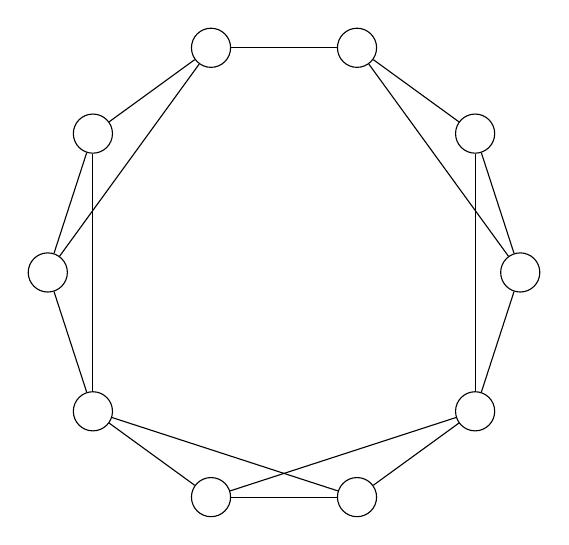
\begin{tikzpicture}

            \newcount \c
            \foreach \n in {0, ..., 9}{
                \c=\n
                \multiply\c by -36
                \advance\c by 90
                \advance\c by 18
                \node[draw, circle, inner sep=5pt, font=\large] (N\n) at (\the\c:3) {~};
            }

            \draw (N0) -- (N1);
            \draw (N1) -- (N2);
            \draw (N1) -- (N3);
            \draw (N2) -- (N3);
            \draw (N2) -- (N4);
            \draw (N3) -- (N4);
            \draw (N4) -- (N5);
            \draw (N4) -- (N6);
            \draw (N5) -- (N6);
            \draw (N5) -- (N7);
            \draw (N6) -- (N7);
            \draw (N7) -- (N8);
            \draw (N7) -- (N9);
            \draw (N8) -- (N0);
            \draw (N8) -- (N9);
            \draw (N9) -- (N0);

        \end{tikzpicture}
        \end{center}
    }

    \only<3>{
        \begin{itemize}
            \item Often, only a few of the decision problems are difficult, so we get very poor
                balance.
        \end{itemize}
    }
\end{frame}

\begin{frame}{Parallel Portfolios?}
    \begin{itemize}
        \item We may have many choices available:
            \begin{itemize}
                \item Models
                \item Heuristics
                \item Search algorithms
                \item Levels of consistency
                \item Solvers
            \end{itemize}

        \item What if we try lots of different combinations in parallel, and pick whichever finishes
            first?
    \end{itemize}
\end{frame}

\begin{frame}{Parallel Consistency?}
\end{frame}

\begin{frame}{Stronger Consistency?}
\end{frame}

\begin{frame}{Bit Parallelism?}
\end{frame}

\begin{frame}{Fixed Parallel Tree Search?}
\end{frame}

\begin{frame}[b]
    \vfill
    \begin{center}
    \url{http://dcs.gla.ac.uk/~ciaran} \\
    \href{mailto:c.mccreesh.1@research.gla.ac.uk}{\nolinkurl{c.mccreesh.1@research.gla.ac.uk}}
\end{center}
\begin{tikzpicture}[remember picture, overlay]
    \node at (current page.north west) {\begin{tikzpicture}[remember picture, overlay]\fill
    [fill=uofgblue, anchor=north west] (0, 0) rectangle (\paperwidth, -1.5cm);\end{tikzpicture}};
    \node [anchor=north west, shift={(0.2cm,-0.2cm)}] at (current page.north west) {\includegraphics*[keepaspectratio=true,scale=0.5]{UoG_keyline.eps}};
\end{tikzpicture}
\end{frame}

\end{document}


